\documentclass[../main.tex]{subfiles}

\begin{document}

Firstly, there will be an endpoint handler handling all \textit{POST} requests at the path \textit{/external-to-internal}.

The endpoint will not contain any business functionality but will delegate the computation to the underlying service. Once the service responds with the result, the endpoint simply returns the resulting DTO.

The above word description is visualized in Figure \ref{fig:translation-design}.

Translation operation can be synchronous since consisting only of parsing, validation, and final concatenation (none of which takes a non-trivial amount of time).

\begin{figure}
  \begin{center}
    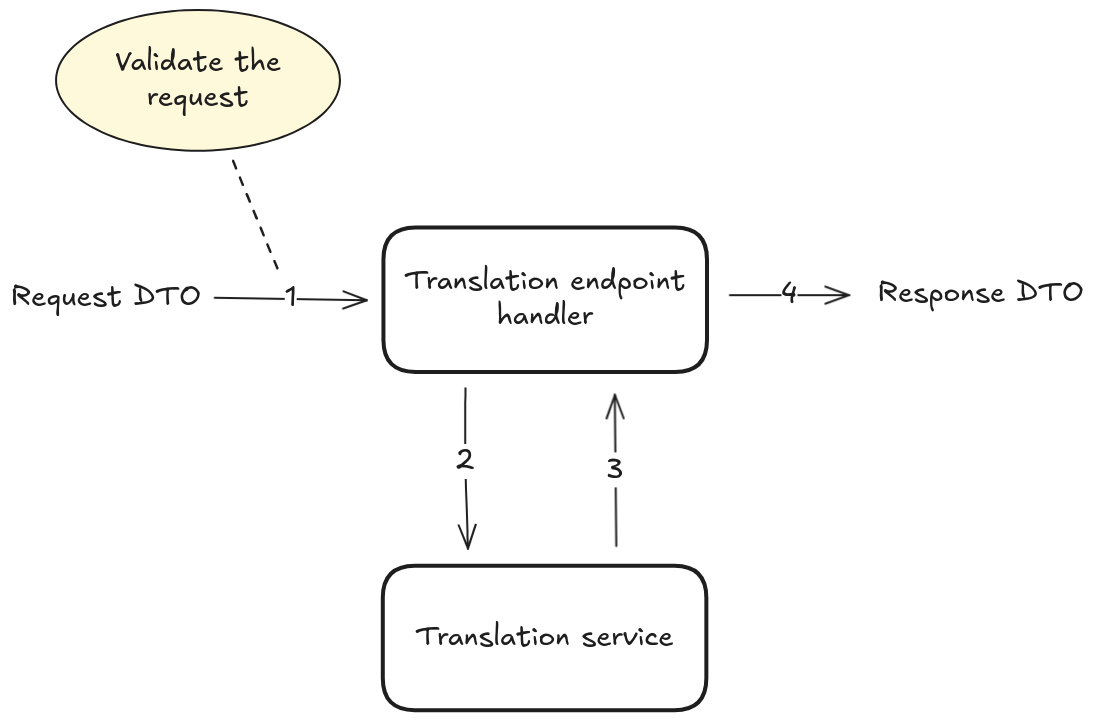
\includegraphics[width=0.8\textwidth]{images/translation-design.png}
  \end{center}
  \caption{Translation design}
  \label{fig:translation-design}
\end{figure}

\end{document}
